% Left: the game of epsilon and N for u_n = 1 + (-1)^n/n. Right: peaks of a bounded sequence (Bolzano-Weierstrass). Generated by figs_t0c05.py.
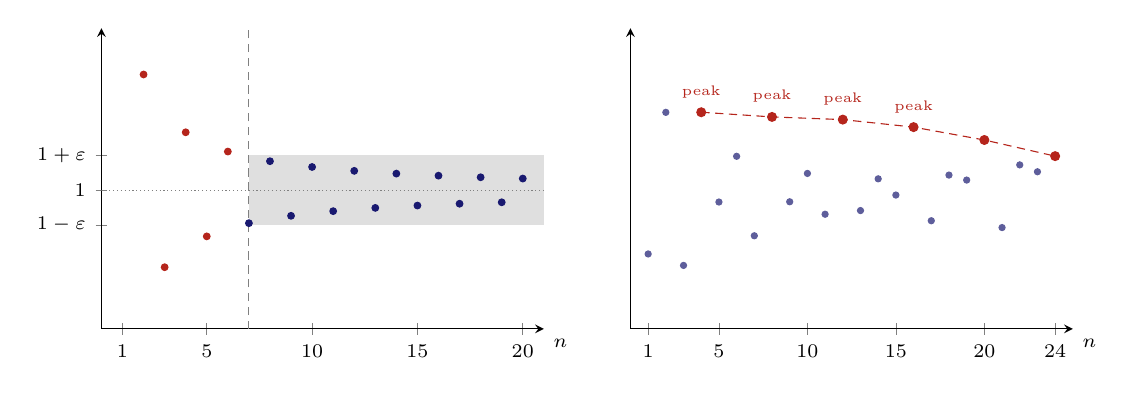
\begin{tikzpicture}
\begin{axis}[name=L,width=7.2cm,height=5.4cm,xmin=0,xmax=21,ymin=0.4,ymax=1.7,axis lines=left,xtick={1,5,10,15,20},ytick={0.85,1,1.15},yticklabels={$1-\varepsilon$,$1$,$1+\varepsilon$},tick label style={font=\scriptsize},xlabel={$n$},xlabel style={font=\scriptsize,at={(1,0)},anchor=north west}]
\fill[gray!25] (axis cs:7,0.85) rectangle (axis cs:21,1.15);
\draw[gray,densely dotted] (axis cs:0,1) -- (axis cs:21,1);
\draw[gray,densely dashed] (axis cs:7,0.4) -- (axis cs:7,1.7);
\node[font=\scriptsize,anchor=north] at (axis cs:7,0.4) {$N=7$};
\addplot[only marks,mark=*,mark size=1.2pt,BrickRed] coordinates {(1.0000,0.0000) (2.0000,1.5000) (3.0000,0.6667) (4.0000,1.2500) (5.0000,0.8000) (6.0000,1.1667)};
\addplot[only marks,mark=*,mark size=1.2pt,MidnightBlue] coordinates {(7.0000,0.8571) (8.0000,1.1250) (9.0000,0.8889) (10.0000,1.1000) (11.0000,0.9091) (12.0000,1.0833) (13.0000,0.9231) (14.0000,1.0714) (15.0000,0.9333) (16.0000,1.0625) (17.0000,0.9412) (18.0000,1.0556) (19.0000,0.9474) (20.0000,1.0500)};
\end{axis}
\begin{axis}[at={(L.east)},anchor=west,xshift=1.1cm,width=7.2cm,height=5.4cm,xmin=0,xmax=25,ymin=-0.3,ymax=2.3,axis lines=left,xtick={1,5,10,15,20,24},ytick=\empty,tick label style={font=\scriptsize},xlabel={$n$},xlabel style={font=\scriptsize,at={(1,0)},anchor=north west}]
\addplot[only marks,mark=*,mark size=1.1pt,MidnightBlue!70] coordinates {(1.0000,0.3479) (2.0000,1.5725) (3.0000,0.2489) (4.0000,1.5735) (5.0000,0.7971) (6.0000,1.1925) (7.0000,0.5053) (8.0000,1.5330) (9.0000,0.7992) (10.0000,1.0443) (11.0000,0.6914) (12.0000,1.5098) (13.0000,0.7232) (14.0000,0.9976) (15.0000,0.8574) (16.0000,1.4448) (17.0000,0.6353) (18.0000,1.0300) (19.0000,0.9869) (20.0000,1.3335) (21.0000,0.5762) (22.0000,1.1182) (23.0000,1.0587) (24.0000,1.1939)};
\addplot[only marks,mark=*,mark size=1.6pt,BrickRed] coordinates {(4.0000,1.5735) (8.0000,1.5330) (12.0000,1.5098) (16.0000,1.4448) (20.0000,1.3335) (24.0000,1.1939)};
\addplot[BrickRed,thin,densely dashed] coordinates {(4.0000,1.5735) (8.0000,1.5330) (12.0000,1.5098) (16.0000,1.4448) (20.0000,1.3335) (24.0000,1.1939)};
\node[font=\tiny,BrickRed,anchor=south] at (axis cs:4,1.614) {peak};
\node[font=\tiny,BrickRed,anchor=south] at (axis cs:8,1.573) {peak};
\node[font=\tiny,BrickRed,anchor=south] at (axis cs:12,1.550) {peak};
\node[font=\tiny,BrickRed,anchor=south] at (axis cs:16,1.485) {peak};
\end{axis}
\end{tikzpicture}
